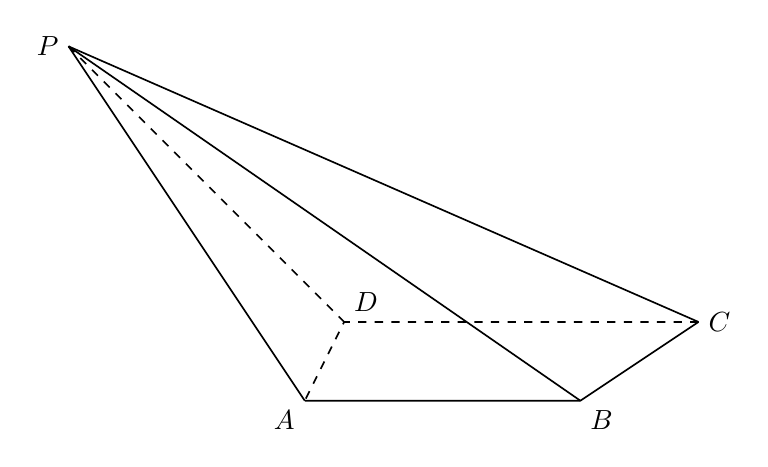
\begin{tikzpicture}[x=1cm,y=1cm,font=\normalsize,line width=.6pt]
\coordinate (P) at (-3.5,4.5);
\coordinate (D) at (0,1.0);
\coordinate (A) at (-0.5,0);
\coordinate (B) at (3.0,0);
\coordinate (C) at (4.5,1.0);
% base rectangle: front solid, back dashed
\draw (A) -- (B) -- (C);
\draw[dashed] (C) -- (D) -- (A);
% lateral edges
\draw (P) -- (A);
\draw (P) -- (B);
\draw (P) -- (C);
\draw[dashed] (P) -- (D);
\node[left] at (P) {$P$};
\node[above right] at (D) {$D$};
\node[below left] at (A) {$A$};
\node[below right] at (B) {$B$};
\node[right] at (C) {$C$};
\end{tikzpicture}
